\documentclass[runningheads]{llncs}

\usepackage[T1]{fontenc}
\usepackage{graphicx}
\usepackage{amsmath}
\usepackage[colorlinks=true,linkcolor=black,citecolor=black,urlcolor=black]{hyperref}

\begin{document}

\title{Characterizing Extended Kalman Filter Fusion of Visual Detection and Odometry Under Sparse Observation: A Multi-Robot Digital Twin Case Study}

\titlerunning{EKF Fusion Under Sparse Observation}

% Camera-ready version — authorship restored post-acceptance.
% This file is NOT the double-blind submission; see main.tex for that.
\author{Yan Santos Leite \and Alisson Assis Cardoso}

\authorrunning{Y. S. Leite and A. A. Cardoso}

\institute{School of Electrical, Mechanical and Computer Engineering,
Universidade Federal de Goiás (UFG), Goiânia, Brazil \\
\email{santosleiteyan@gmail.com}, \email{alsnac@ufg.br}}

\maketitle

\begin{abstract}
Multi-robot systems combining odometry with external visual detection
often rely on a discrete fallback — trusting detection when available,
odometry otherwise — which discards uncertainty information and offers
no principled behavior during long detection gaps. We replace this
fallback with a per-robot Extended Kalman Filter fusing odometry and
YOLO-based visual detection from a fixed overhead camera, validated in
two stages (synthetic NEES/NIS consistency, then real recorded data) on
a ROS2/Gazebo digital twin using three TurtleBot3 robots. Measured at
correction instants, the filter reduces position error by $+23.7\%$
relative to odometry alone under aggressive drift. However, measured
continuously — at every odometry reading — the same filter is $12.7\%$
\emph{worse} than raw odometry, under the sparse visual coverage
(0--28\%) our camera setup exhibits in practice. We show this reversal
is the expected consequence of operating below a critical observation
rate, not a design flaw, and connect it mechanistically to a covariance
ceiling required to keep Mahalanobis-gated association stable. We argue
that reporting both metrics, rather than only the commonly reported
correction-instant gain, is necessary to honestly characterize EKF
fusion under sparse observation, and discuss why alternative filters
(UKF, particle filter, IMM) do not resolve the underlying limitation.

\keywords{Extended Kalman Filter \and Sensor Fusion \and Multi-Robot Localization \and Sparse Observations \and Digital Twin}
\end{abstract}

\section{Introduction}

Multi-robot systems combining onboard odometry with external visual
detection face a recurring choice: how to combine two noisy position
estimates arriving at different rates, not always available at the same
instant. A common, pragmatic solution — used in the digital twin studied
here prior to our contribution — is a \emph{discrete fallback}: trust
detection when confidently associated, odometry otherwise. This is
simple and robust but discards information: no partial correction from
low-confidence detections, no uncertainty propagation, and no principled
behavior during long detection-free stretches.

Extended Kalman Filtering (EKF) is the classical answer, offering full
probabilistic prediction/correction with explicit uncertainty
propagation. Its convergence properties, however, are classically
established under reasonably dense, regular
observation~\cite{dissanayake2001slam} — an assumption a single fixed
overhead camera, subject to finite field of view and self-occlusion
during maneuvers, does not generally satisfy. Whether this matters in
practice, on a real platform rather than only in simulation, is the
question this paper investigates.

We replace the discrete fallback with a per-robot EKF fusing odometry
and YOLO-based visual detection, evaluated end-to-end on a ROS2/Gazebo
digital twin with three TurtleBot3 robots. Our contribution is
twofold. First, validated in two stages (synthetic NEES/NIS, then real
recorded data), the filter delivers a real fusion gain ($+23.7\%$
position error reduction relative to odometry alone, under aggressive
drift, at correction instants). Second, and more centrally, the same
filter measured continuously — not only at correction
instants — is $12.7\%$ \emph{worse} than raw odometry under the sparse
visual coverage (0--28\%) our camera exhibits in practice. We explain
this reversal mechanistically, connecting it to established theory on
Kalman filtering under intermittent
observations~\cite{sinopoli2004intermittent,censi2009geometric}, and
argue that reporting both metrics — not only the commonly reported
correction-instant gain — is necessary for honest characterization, and
discuss why alternative filters do not resolve the underlying
limitation.

\section{Related Work}
\label{sec:related-work}

Bailey and Durrant-Whyte~\cite{bailey2006slam} formalize the standard EKF
motion/observation model our filter follows directly (odometry drives
prediction, YOLO detections drive correction; notation adopted in
Section~\ref{sec:methodology}). Dissanayake et
al.~\cite{dissanayake2001slam} prove EKF-SLAM covariance convergence
under \emph{dense} landmark observation — an assumption our
0--28\%-coverage overhead camera violates by construction, which is
central to Section~\ref{sec:discussion}. Sinopoli et
al.~\cite{sinopoli2004intermittent} establish that, under Bernoulli
observation arrival, covariance diverges below a critical rate; our
Scenario~3 (0\% coverage) sits at the limiting case $p\to0$, so the
saturation we observe is theoretically expected, not a symptom of
misconfiguration. Censi~\cite{censi2009geometric} notes this critical
threshold depends on the covariance summary metric used; we report
$\mathrm{trace}(P)$ as a scoping choice, not a claim of
metric-independence.

Khosravi et al.~\cite{khosravi2026cooperative} report decentralized
cooperative localization for two robots (mutual LiDAR corrections,
Gazebo and hardware), with $34$--$56\%$ RMSE reduction — comparable in
order of magnitude to our $+23.7\%$. Ahmed and
Fr\'emont~\cite{ahmed2026maritime} fuse a custom YOLOv8-RGBDis detector
with a per-target EKF for a maritime multi-robot team, reporting
$\mathrm{mAP@0.5}=0.995$, numerically close to ours despite different
architecture/domain. Neither reports a continuous-error regime in which
fusion underperforms the unfused baseline — the differentiating finding
of this work. Dobrynin and Garcia~\cite{dobrynin2025turtlebot} share our
exact platform (three TurtleBot3, ROS2) but solve camera-free relative
localization, so do not encounter sparse visual coverage; we revisit
this as complementary work in Section~\ref{sec:future-work}. Our
contribution is the joint report of both the correction-instant gain and
the continuous-error degradation, grounded in
\cite{sinopoli2004intermittent,censi2009geometric} for why this
trade-off is expected rather than an implementation bug.

\section{Methodology}
\label{sec:methodology}

Following Bailey and Durrant-Whyte~\cite{bailey2006slam}, each robot is
tracked by an independent EKF with state $x_k=[p_x,p_y,\theta]^\top$.
The motion model integrates the \emph{delta} of consecutive odometry
readings onto the current state — not the absolute value, which would
discard prior visual corrections. The observation model maps state to
the 2D position reported by a YOLO detector on a fixed overhead camera
(Section~\ref{sec:experimental-setup}).

\textbf{Prediction and covariance capping.} Process noise is
$Q=\mathrm{diag}(0.5,0.5,0.25)$, scaled by $\Delta t/0.1$ for the real
odometry rate ($\approx$29\,Hz vs.\ the 0.1s assumed during synthetic
calibration); calibrated empirically against real data (a sweep from
$10^{-6}$ to $1.0$ showed monotonically increasing gain up to saturation
at $Q\ge0.5$). A hard ceiling $\mathrm{clip}(P,-\infty,0.05)$
(element-wise) is applied after each prediction: without it, $P$ grew
unbounded during long uncorrected intervals (observed
$\mathrm{trace}(P)\approx85$ vs.\ an expected $\approx0.5$), breaking
Mahalanobis-gated association by widening a robot's acceptance region
enough to claim a neighbor's detection. This is functionally analogous
to \emph{track coasting} in multi-target tracking (Bar-Shalom), and
theoretically motivated by Sinopoli et
al.'s~\cite{sinopoli2004intermittent} covariance-divergence result — it
trades strict optimality for bounded, predictable behavior under the
sparse-observation regime we operate in. We report the ceiling's effect
on continuous-time error explicitly in Section~\ref{sec:results}, not as
an implementation detail.

\textbf{Correction.} Measurement noise $R$ is derived linearly from YOLO
detection confidence $c\in[0,1]$ (carried in the otherwise-unused $z$
component of each detected pose), $\sigma=R_{\min}+(1-c)(R_{\max}-R_{\min})$,
$R_{\min}=0.02$, $R_{\max}=0.20$\,m — a high-confidence detection is
trusted more during the Kalman update.

\textbf{Data association.}
\label{sec:association}
With up to three robots visible simultaneously, each detection is
assigned via Mahalanobis-gated nearest-neighbor: $d^2=e^\top P_{xy}^{-1}e$
per (robot, detection) pair, accepted only if $d^2\le9.21$ (99\%
confidence, $\chi^2$, 2 DOF). This inherits a known limitation
(Altendorfer and Wirkert~\cite{altendorfer2016association}): an inflated
covariance widens the acceptance region and can bias association toward
more uncertain tracks — the same failure mode motivating the covariance
ceiling above.

\textbf{Camera calibration.} Intrinsics come from
\texttt{cv2.calibrateCamera} (Zhang~\cite{zhang2000calibration}) using a
synthetic checkerboard at multiple poses, with a sanity check rejecting
low-reprojection-error but ill-conditioned solutions (focal length far
from the FOV-derived theoretical value) — accepted calibration:
$f_x=739.4$, $f_y=733.6$, mean reprojection error 0.162px.

\textbf{Two-stage validation.} (1) Synthetic NEES/NIS: 30 Monte Carlo
seeds (2000 steps each) give NEES$=2.955$ (expected $3.0$) and
NIS$=1.982$ (expected $2.0$), within 1.5\%/0.9\% relative error —
well-calibrated in practice despite formal $\chi^2$ 95\% bounds being
too narrow to pass at this sample size. (2) The calibrated filter is
then run against real odometry and YOLO detections recorded from the
live digital twin, where observation coverage is sparse and irregular
by construction of the physical scenario, not by design choice.

\section{Experimental Setup}
\label{sec:experimental-setup}

We evaluate our EKF in a ROS2/Gazebo digital twin: three TurtleBot3
Waffle units in a shared simulated world alongside a static overhead
camera at $(0,0,3)$\,m, $90^\circ$ downward pitch, $60^\circ$ horizontal
FOV, publishing $640\times480$ frames at 10\,Hz. Each robot also
publishes odometry ($\approx$29\,Hz) and an unused 2D LiDAR scan
(Section~\ref{sec:future-work}). Robot detection uses a YOLO model
trained on 375 annotated frames from the same camera,
$\mathrm{mAP@0.5}=0.995$ on held-out validation; confidence is carried
in the detection message's otherwise-unused $z$ field for direct
consumption by the EKF correction step.

Three $\sim$18\,s scenarios were recorded as ROS2/MCAP bags: (a)
\textbf{Stationary} — 152 detections vs.\ 550 odometry readings/robot,
$\approx$28\% coverage, the highest of the three; (b) \textbf{Straight
motion} ($v_x=0.1$\,m/s) — 144 vs.\ 522 readings, $\approx$11\%
coverage, $\sim$1.5\,m confirmed ground-truth displacement; (c)
\textbf{Curve/occlusion} ($v_x=0.12$\,m/s, $\omega_z=0.4$\,rad/s) — 145
detections recorded on the topic, but \textbf{zero} successfully
associated to \texttt{robot1} over the full recording: the single fixed
viewpoint loses robots to self-occlusion and out-of-frame motion during
turns, producing the 0\% coverage case central to
Section~\ref{sec:results}. Timestamp synchronization between detections
and odometry was verified via \texttt{rosbag2\_py} in all three
scenarios (no gap $>$500\,ms on any channel), ruling out sensor-clock
desynchronization as a confound.

We release a reproducibility package (world file, URDF, calibration,
EKF hyperparameters, code commit SHA) supporting independent
verification, and document one non-obvious dependency:
\texttt{ros-humble-rosbag2-storage-mcap} is not installed by default on
ROS2 Humble.

\section{Results}
\label{sec:results}

We report two distinct error metrics, deliberately kept separate rather
than collapsed into a single number: \emph{correction-instant error},
measured only at the moments a YOLO detection is successfully associated
and fused (the metric most commonly reported in related
work — Section~\ref{sec:related-work}), and \emph{continuous error},
measured at every odometry reading regardless of whether a correction
occurred. As we show below, these two metrics disagree in sign, and both
are necessary to honestly characterize the filter's behavior under
sparse observation.

\subsection{Filter Calibration}

The synthetic NEES/NIS validation described in
Section~\ref{sec:methodology} confirms the filter is well-calibrated
before any real-data evaluation. Fig.~\ref{fig:nees-nis} shows both
statistics remaining close to their theoretical expected values
(NEES$\to 3.0$, NIS$\to 2.0$) across the Monte Carlo run.

\begin{figure}[htbp]
\centering
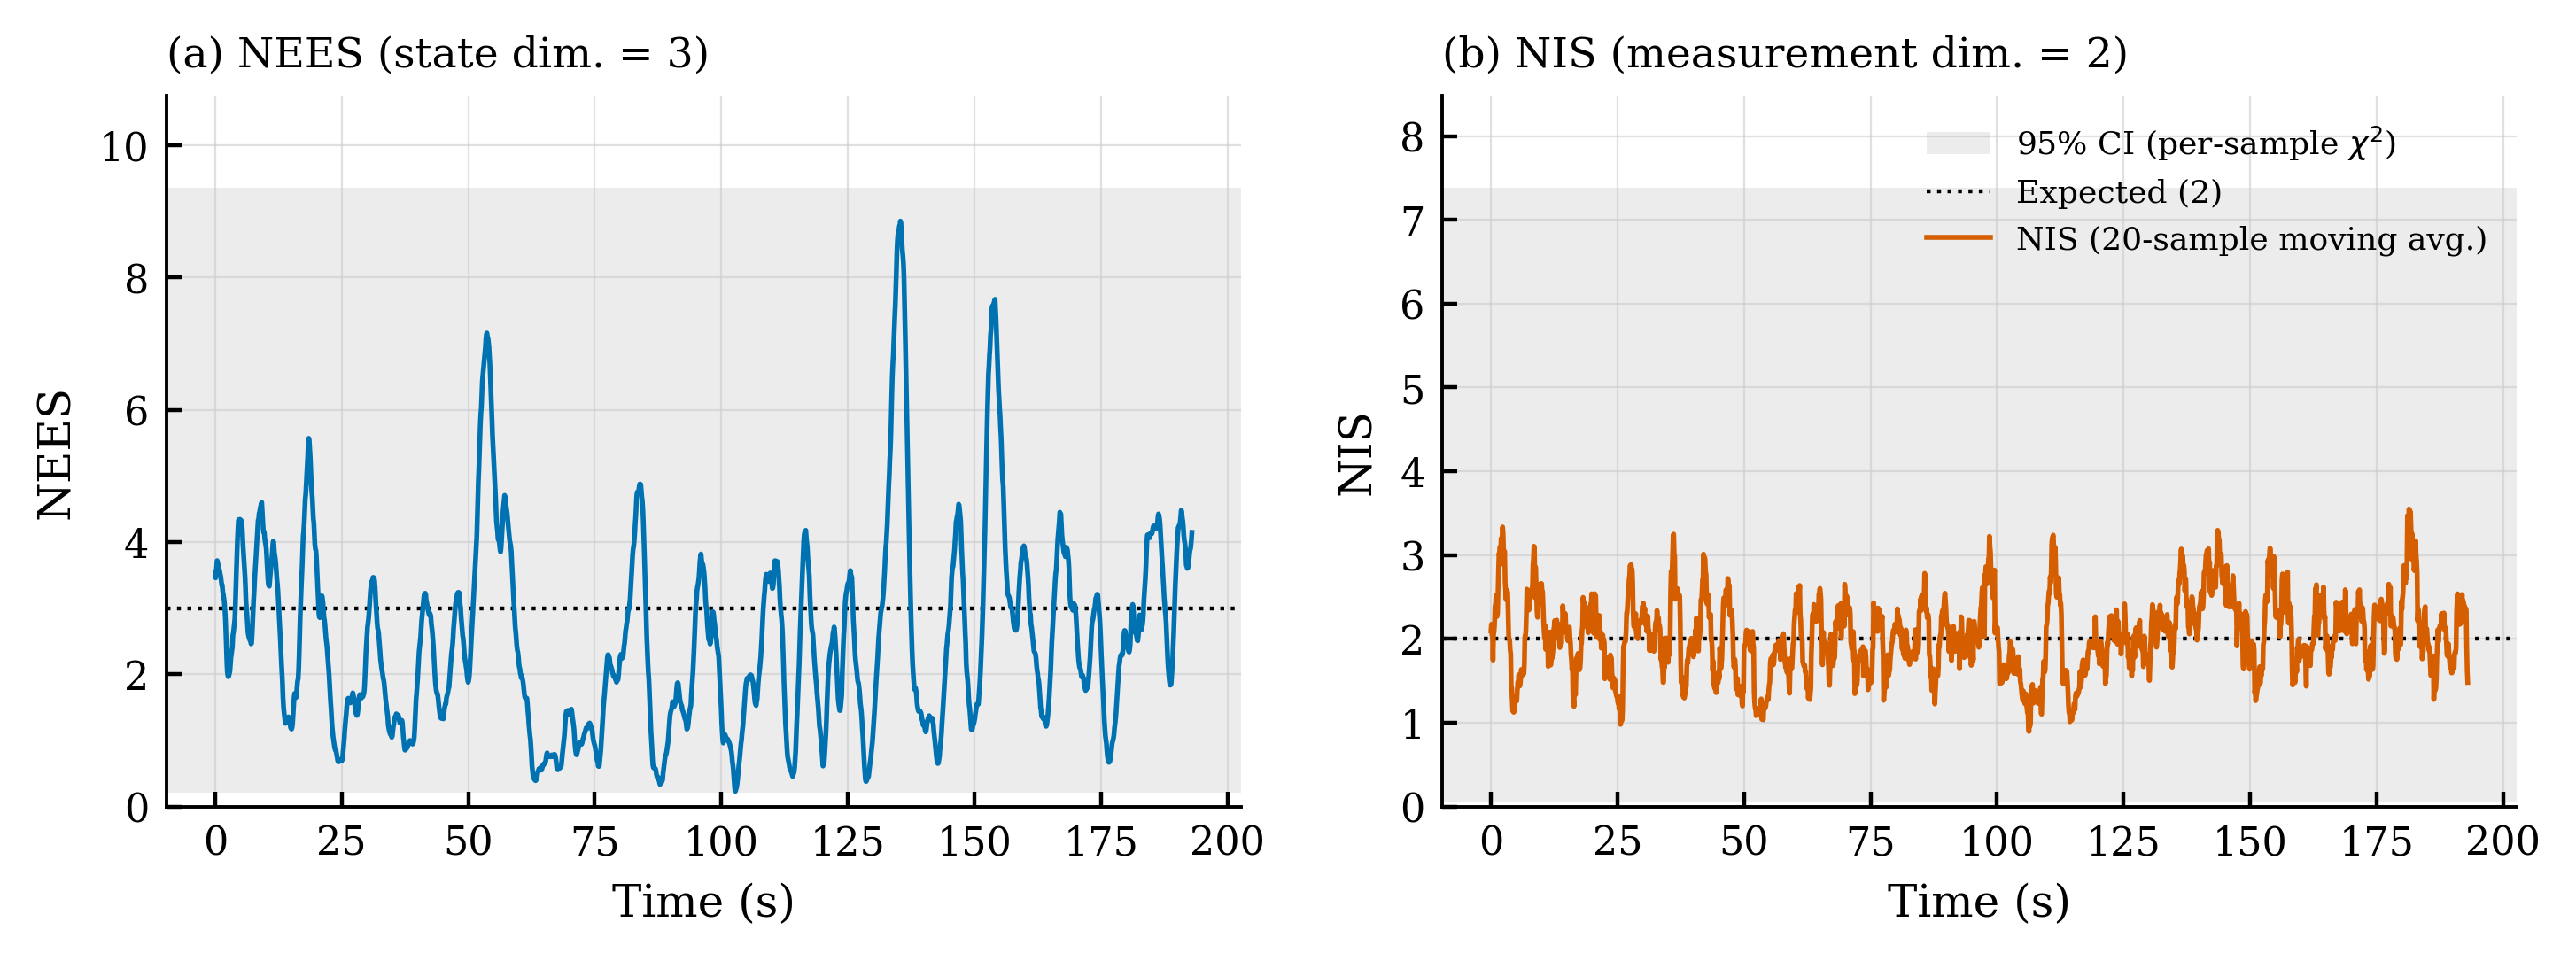
\includegraphics[width=0.85\textwidth]{../lafusion/figures/lafusion_nees_nis.png}
\caption{NEES and NIS consistency over the synthetic Monte Carlo
validation (30 seeds, 2000 steps each). Both statistics track their
theoretical expected values, indicating a well-calibrated filter.}
\label{fig:nees-nis}
\end{figure}

\subsection{Correction-Instant Error}

Table~\ref{tab:correction-error} reports position error under three
injected odometry drift regimes (no drift, light drift, aggressive
drift), aggregated across all three recorded scenarios ($n=1323$). Under
aggressive drift — the regime in which raw odometry has already
accumulated substantial error before a visual correction becomes
available — the EKF reduces mean position error by $+23.7\%$ relative to
odometry alone (Wilcoxon signed-rank, $p<0.001$). Under light drift, the
gain is negative ($-5.3\%$): visual detection error ($\approx$3--6\,cm)
is not yet smaller than the still-small odometry error, so fusion offers
no benefit in this regime — expected behavior for a correctly calibrated
filter, not a failure.

\begin{table}
\caption{Correction-instant position error (m), aggregated over 3
scenarios ($n=1323$).}\label{tab:correction-error}
\begin{tabular}{|l|c|c|c|}
\hline
\textbf{Drift regime} & \textbf{EKF (mean)} & \textbf{Odom-only (mean)} & \textbf{Change} \\
\hline
None (odom = GT by construction) & 0.0356 & 0.0000 & N/A \\
\hline
Light & 0.0528 & 0.0501 & $-5.3\%$ \\
\hline
Aggressive & 0.1282 & 0.1681 & $\mathbf{+23.7\%}$ \\
\hline
\end{tabular}
\end{table}

\begin{figure}[htbp]
\centering
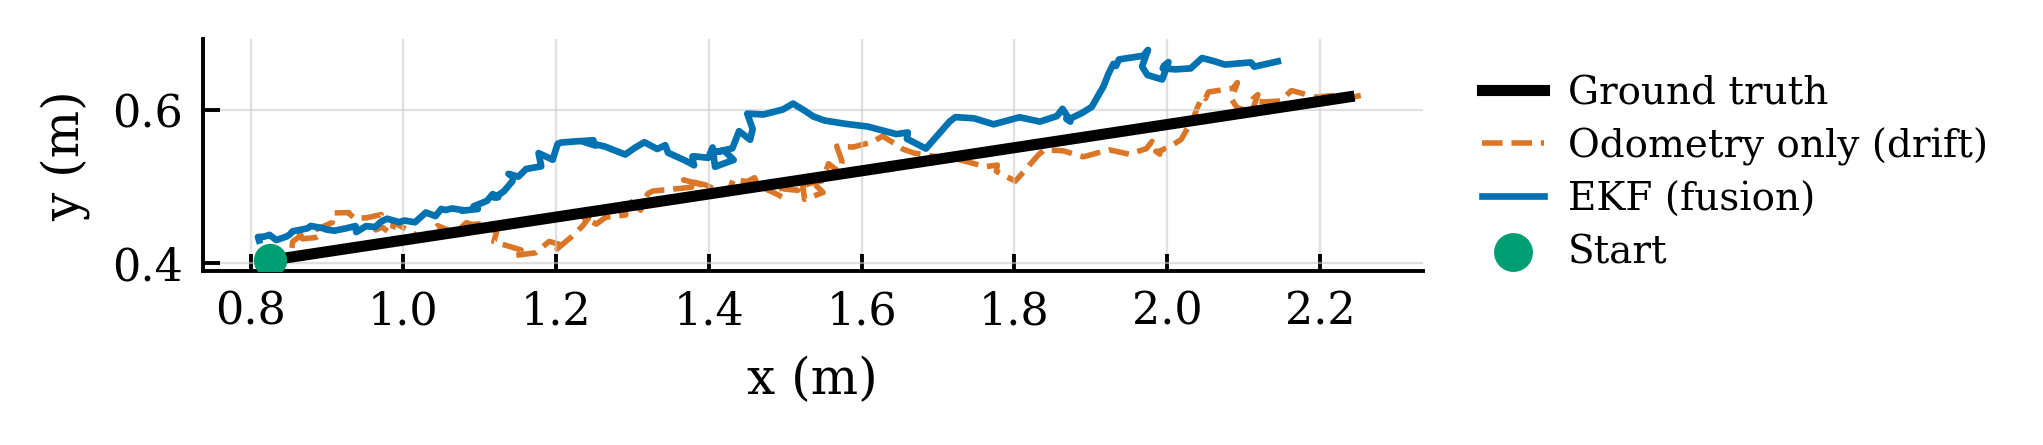
\includegraphics[width=0.6\textwidth]{../lafusion/figures/lafusion_trajectory.png}
\caption{Estimated trajectory under aggressive drift, Scenario 2
(straight motion). The EKF (blue) tracks ground truth (black) more
closely than raw drifted odometry (orange, dashed).}
\label{fig:trajectory}
\end{figure}

Fig.~\ref{fig:trajectory} shows this qualitatively: raw odometry visibly
drifts from the straight ground-truth path, while the EKF estimate
tracks it more closely.

\subsection{Continuous Error: The Central Finding}

When error is instead measured at \emph{every} odometry reading — not
only at correction instants — the result reverses. Table~\ref{tab:continuous-error}
reports continuous-time error under aggressive drift, using the same
recordings as Table~\ref{tab:correction-error}. Aggregated across all
readings ($n=1607$), the EKF is $12.7\%$ \emph{worse} than raw odometry
(Wilcoxon signed-rank, $p<0.001$) — the opposite sign from the
correction-instant result.

\begin{table}
\caption{Continuous position error (m), every odometry reading,
aggressive drift.}\label{tab:continuous-error}
\begin{tabular}{|l|c|c|c|c|}
\hline
\textbf{Scenario} & \textbf{YOLO coverage} & \textbf{EKF (mean)} & \textbf{Odom-only (mean)} & \textbf{Change} \\
\hline
Stationary & 27.6\% & 0.2116 & 0.1774 & $-19.3\%$ \\
\hline
Straight motion & 11.3\% & 0.2115 & 0.1780 & $-18.8\%$ \\
\hline
Curve / occlusion & 0.0\% & 0.1778 & 0.1778 & $-0.0\%$ \\
\hline
\textbf{Aggregated} & --- & \textbf{0.2003} & \textbf{0.1777} & $\mathbf{-12.7\%}$ \\
\hline
\end{tabular}
\end{table}

Two observations explain this reversal. First, the degradation scales
inversely with YOLO coverage: Scenario 3 (0\% coverage — no successful
visual correction over the entire $\sim$18\,s recording) shows a change
of exactly $0.0\%$, because with zero corrections the EKF's prediction
step degenerates to pure odometry-delta integration, making it
mathematically identical to the unfused baseline. Scenarios 1 and 2
(27.6\% and 11.3\% coverage) show similar $\sim$19\% degradation despite
their different coverage levels, suggesting the effect saturates quickly
once corrections become sparse enough for the covariance ceiling
(Section~\ref{sec:methodology}) to bind.

\begin{figure}[htbp]
\centering
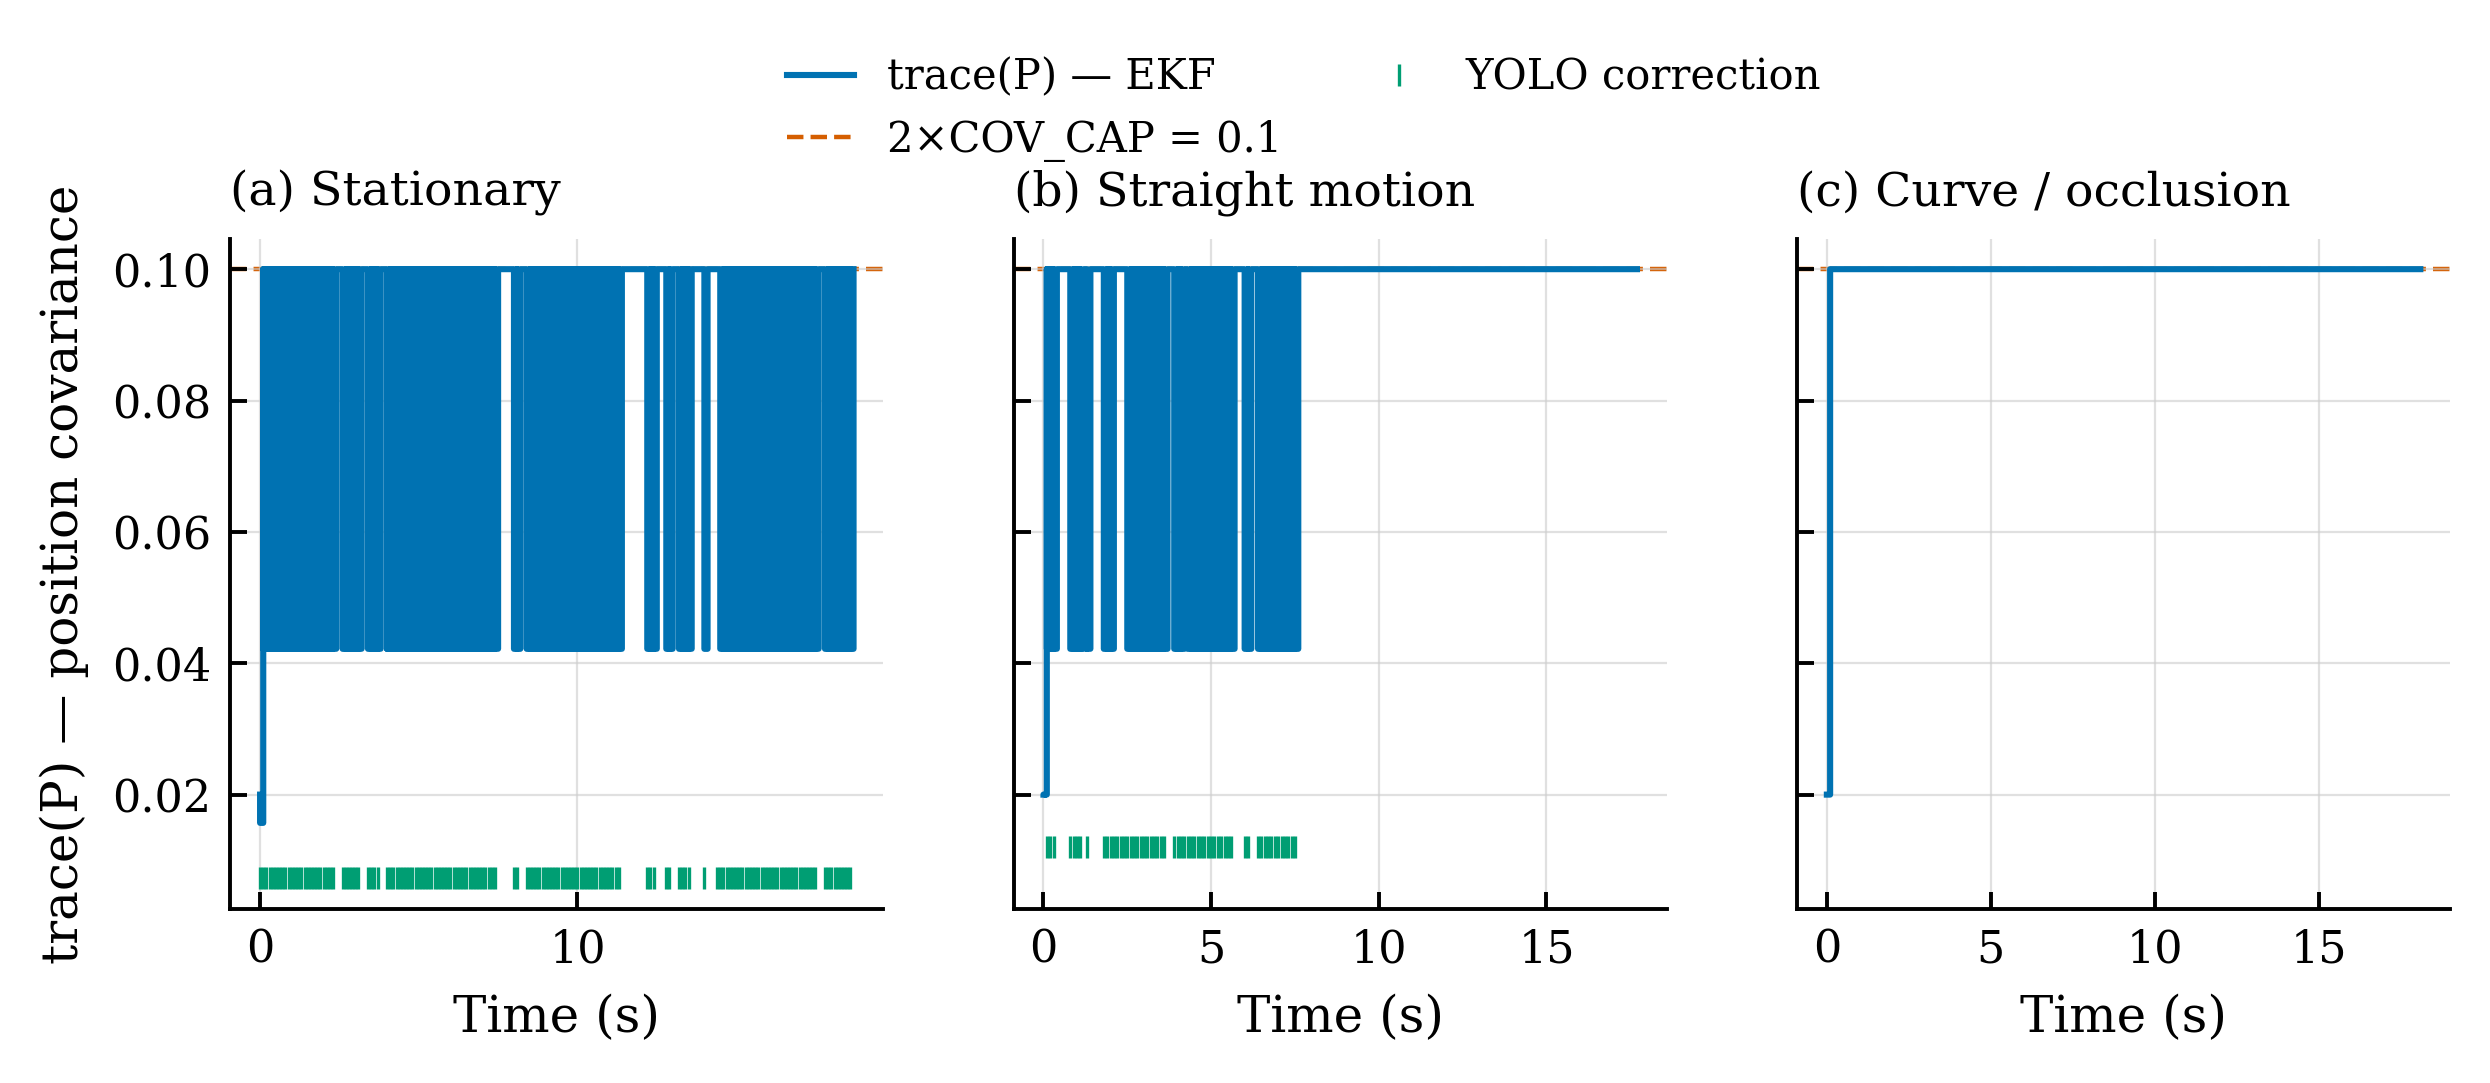
\includegraphics[width=0.72\textwidth]{../lafusion/figures/lafusion_covariance_trace.png}
\caption{$\mathrm{trace}(P_{xy})$ over time (step plot), all three
scenarios. Short vertical ticks along the bottom mark successful YOLO
corrections. The dashed line marks $2\times\mathrm{COV\_CAP}=0.1$, the
ceiling on the position-covariance trace (Section~\ref{sec:methodology}).
Coverage decreases left to right (27.6\% $\to$ 11.3\% $\to$ 0\%), and
covariance saturates at the ceiling for correspondingly longer
stretches, reaching permanent saturation in the zero-coverage case.}
\label{fig:covariance-trace}
\end{figure}

Second, and mechanistically explaining the first, Fig.~\ref{fig:covariance-trace}
shows why: $\mathrm{trace}(P)$ saturates at the covariance ceiling almost
immediately after any gap without correction, and only drops when a
correction lands. In Scenario 3, the trace saturates within the first
observed step and never drops again for the remainder of the recording.
This is precisely the divergence regime predicted by Sinopoli et
al.~\cite{sinopoli2004intermittent} for observation arrival rates below a
critical threshold: the filter's covariance ceiling prevents unbounded
growth (and the association failures it would otherwise cause,
Section~\ref{sec:methodology}), but it does so by capping the filter's
\emph{own estimate of its uncertainty}, not by making its state estimate
actually more accurate during the uncorrected interval — the filter
remains overconfident in its odometry-only prediction relative to how
uncertain that prediction actually is.

\section{Discussion}
\label{sec:discussion}

The natural reading of Table~\ref{tab:continuous-error} is unflattering:
our EKF, evaluated continuously, loses to the odometry it should
improve upon. We argue this is expected, not a flawed design.
Dissanayake et al.'s~\cite{dissanayake2001slam} convergence proof
assumes dense observation; our camera violates that by construction
(0--28\% coverage), and Sinopoli et al.~\cite{sinopoli2004intermittent}
predict exactly this covariance divergence without a ceiling, and
resulting overconfidence with one. Scenario~3's $0.0\%$ change is a
clean confirmation: with zero corrections, the filter's prediction step
is provably identical to odometry-delta integration. We follow
Censi~\cite{censi2009geometric} in reporting $\mathrm{trace}(P)$ as a
scoping choice, not a claim of metric-independent divergence.

No standard alternative resolves the zero-coverage case: a particle
filter degenerates to pure process propagation with no likelihood to
reweight against; a UKF targets observation-model nonlinearity, not
observation \emph{rate} (our near-linear projection gains little); an
IMM filter still requires some observation to weight competing modes.
We treat low coverage — a single fixed viewpoint subject to
occlusion — as the root cause, consistent with sensor-placement
literature: estimation limits under a given sensor topology hold
independently of the filter used. The covariance ceiling is thus an
engineering approximation of \emph{track coasting} (Bar-Shalom),
trading optimality for association stability, and inherits a known gating
limitation (Altendorfer and
Wirkert~\cite{altendorfer2016association}): a saturated covariance
widens the acceptance region precisely when true uncertainty is least
well characterized by a fixed value — though we did not observe
incorrect cross-robot association in our three scenarios.

\section{Future Work}
\label{sec:future-work}

Concrete directions include: (a) \textbf{adaptive process noise} — scale
$Q$ by time since the last correction instead of a fixed ceiling, more
principled at the cost of an added hyperparameter; (b) \textbf{LiDAR as
a third fusion source} — each robot already publishes unused 2D scans;
mutual LiDAR corrections (in the spirit of
Khosravi et al.~\cite{khosravi2026cooperative}) could target the
zero-coverage regime directly; (c) \textbf{formal projection
uncertainty} — propagate the full projection Jacobian (calibration
error, ground-plane assumption) into $R$; (d) \textbf{combining with
distributed relative localization} — Dobrynin and
Garcia's~\cite{dobrynin2025turtlebot} camera-free distributed filtering
on the same platform could provide a second correction channel
available during visual-coverage gaps.

\section{Conclusion}

We replaced a discrete visual/odometry fallback with a two-stage
validated Extended Kalman Filter, evaluated on real recorded data from
three TurtleBot3 robots. The filter delivers a genuine gain at
correction instants ($+23.7\%$) but is measurably worse than raw
odometry when evaluated continuously ($-12.7\%$) under 0--28\% visual
coverage — including a zero-coverage scenario collapsing, exactly as
expected, to the unfused baseline. Rather than report only the
favorable metric, we characterize both and ground the reversal in
established theory on intermittent-observation Kalman filtering. EKF
fusion remains the right tool for this problem, but its correctness
under sparse observation must be measured and reported explicitly, and
the observation rate itself — not the choice of filter — is the binding
constraint future work should target.

\begin{thebibliography}{8}

\bibitem{bailey2006slam}
Bailey, T., Durrant-Whyte, H.: Simultaneous localization and mapping
(SLAM): Part I. IEEE Robotics \& Automation Magazine \textbf{13}(2),
99--110 (2006)

\bibitem{dissanayake2001slam}
Dissanayake, M.W.M.G., Newman, P., Clark, S., Durrant-Whyte, H.F.,
Csorba, M.: A solution to the simultaneous localization and map building
(SLAM) problem. IEEE Transactions on Robotics and Automation
\textbf{17}(3), 229--241 (2001)

\bibitem{sinopoli2004intermittent}
Sinopoli, B., Schenato, L., Franceschetti, M., Poolla, K., Jordan, M.I.,
Sastry, S.S.: Kalman filtering with intermittent observations. IEEE
Transactions on Automatic Control \textbf{49}(9), 1453--1464 (2004)

\bibitem{censi2009geometric}
Censi, A.: Geometric remarks on Kalman filtering with intermittent
observations. arXiv:0906.1637 (2009)

\bibitem{zhang2000calibration}
Zhang, Z.: A flexible new technique for camera calibration. IEEE
Transactions on Pattern Analysis and Machine Intelligence \textbf{22}(11),
1330--1334 (2000)

\bibitem{altendorfer2016association}
Altendorfer, R., Wirkert, S.J.: Why the association log-likelihood
distance should be used for measurement-to-track association. In: 2016
IEEE Intelligent Vehicles Symposium (IV). pp. 258--265 (2016)

\bibitem{khosravi2026cooperative}
Khosravi, N., Khosravi, N., Bozorg, M., Bahraini, M.S.: Decentralized
Cooperative Localization for Multi-Robot Systems with Asynchronous Sensor
Fusion. arXiv:2603.12075 (2026)

\bibitem{ahmed2026maritime}
Ahmed, M.F., Fr\'emont, V.: Decentralized Multi-Robot Obstacle Detection
and Tracking in a Maritime Scenario. arXiv:2602.12012 (2026)

\bibitem{dobrynin2025turtlebot}
Dobrynin, D., Garcia, I.T.: A TurtleBot3 Hardware Testbed for Distributed
Kalman Filter Localization. Senior Project, California Polytechnic State
University, San Luis Obispo (2025)

\end{thebibliography}
\end{document}
